\RequirePackage{pdfmanagement}
\SetKeys[document/metadata]{pdfversion=1.7, pdfstandard=A-2u, lang=en-GB}
\input{preamble/pdfA-compliance/glyphtounicode}
\documentclass[11pt,a4paper]{report}

\newcommand*{\PaperTitle}{Local stability does not imply global stability in the mixed-mechanism phosphorylation network}
\newcommand*{\PaperTitlePlain}{Local stability does not imply global stability in the mixed-mechanism phosphorylation network}
\newcommand*{\PaperShortTitle}{Mixed-mechanism phosphorylation: local is not global}
\newcommand*{\PaperSubtitle}{chemistry-open-problems \textperiodcentered{} 5 November 2026 \textperiodcentered{} preliminary}
\newcommand*{\PaperCredits}{Solver: Claude Opus 5.5 (effort xhigh) \textperiodcentered{} Independent verification: pending}
\newcommand*{\PaperKeywords}{dual-site phosphorylation, mixed mechanism, subcritical Hopf bifurcation, first Lyapunov coefficient, global stability, computer-assisted proof, CAPD}
\input{chemop-preamble}
\addbibresource{references.bib}

\begin{document}
\makepapertitle

\begin{paperabstract}
Conradi, Mincheva and Shiu (Bull.\ Math.\ Biol.\ 2019) studied the dual-site phosphorylation network with processive phosphorylation and distributive dephosphorylation, which has a unique steady state in every compatibility class and loses stability only through Hopf bifurcations. They asked whether a locally stable steady state is always globally stable in its class. It is not. For the integer rate constants $k=(1,1,1,1,300,1,3,1,1,100)$ the Hopf bifurcation along an explicit line of compatibility classes is subcritical: we certify in ball arithmetic a simple pair $\pm i\omega_0$, the other four eigenvalues in the open left half-plane, a positive crossing speed and a positive first Lyapunov coefficient. Hence classes with a locally asymptotically stable steady state contain an unstable periodic orbit. At the rational class $(K_{\rm tot},P_{\rm tot},S_{\rm tot})=(236/3,\,6527/1800,\,341699/5400)$ we prove, by exact arithmetic and a CAPD computer-assisted proof, that the steady state is locally asymptotically stable while the class contains an orbitally asymptotically stable periodic orbit and a second periodic orbit. The same conclusion holds on a nonempty open set of rate constants and total amounts. The conjecture of the same paper, that an unstable steady state always coexists with a stable periodic orbit, is not settled. Our example is consistent with it, and we certify one instance.
\end{paperabstract}

\section*{The question}
Conradi, Mincheva and Shiu~\autocite{CMS2019} (arXiv:1809.02886v2, Section~6, p.~20; journal version Section~6, p.~1849) end their study of the mixed-mechanism network with the question:
\begin{openquote}
``Finally, we consider the dynamics in compatibility classes that contain a locally stable steady state. Our simulations suggest that such a steady state is in fact globally stable. Accordingly, we pose the question, Consider the mixed-mechanism network, and any choice of rate constants and total amounts. If the unique steady state $x^*$ in $\mathcal P$ is locally stable, does it always follow that $x^*$ is globally stable? In the Michaelis-Menten limit, this is true [36].''
\end{openquote}
The same section (arXiv p.~18, journal p.~1848) states, as Conjecture~6.1 in both versions:
\begin{openquote}
``Conjecture 6.1. Consider the mixed-mechanism network, and any choice of rate constants and total amounts. If the unique steady state in $\mathcal P$ is unstable, then $\mathcal P$ contains a stable periodic orbit.''
\end{openquote}
Conjecture~6.2 of~\autocite{CMS2019} is a different statement (persistence of oscillations for large $K_{\rm tot}$). The reference [36] in the quotation is Rao~\autocite{Rao2018}. We answer the question in the negative (\zcref{thm:hopf,thm:explicit,thm:open}); \zcref{sec:conj} discusses what this implies for Conjecture~6.1.

\section{Setting}\label{sec:setting}
\paragraph{The network.} With $x_1,\dots,x_9$ the concentrations of $S_0$, $K$, $S_0K$, $S_1K$, $S_2$, $P$, $S_2P$, $S_1$, $S_1P$, the mass-action system (equation~(2) of~\autocite{CMS2019}) is $\dot x=g(x)=N\,r(x)$, where the ten reactions and rates are
\[
\begin{aligned}
&S_0+K\xrightarrow{k_1}S_0K,\quad S_0K\xrightarrow{k_2}S_0+K,\quad S_0K\xrightarrow{k_3}S_1K,\quad S_1K\xrightarrow{k_4}S_2+K,\\
&S_2+P\xrightarrow{k_5}S_2P,\quad S_2P\xrightarrow{k_6}S_2+P,\quad S_2P\xrightarrow{k_7}S_1+P,\\
&S_1+P\xrightarrow{k_8}S_1P,\quad S_1P\xrightarrow{k_9}S_1+P,\quad S_1P\xrightarrow{k_{10}}S_0+P,
\end{aligned}
\]
$r_1=k_1x_1x_2$, $r_5=k_5x_5x_6$, $r_8=k_8x_6x_8$, and the other $r_j$ are linear. The totals
\[
K_{\rm tot}=x_2+x_3+x_4,\qquad P_{\rm tot}=x_6+x_7+x_9,\qquad S_{\rm tot}=x_1+x_3+x_4+x_5+x_7+x_8+x_9
\]
are conserved; write $T=(K_{\rm tot},P_{\rm tot},S_{\rm tot})=Wx$. The stoichiometric subspace $\mathcal S=\operatorname{im}N=\ker W$ has dimension~6, and the compatibility class of $T\in\mathbb R^3_{>0}$ is $\mathcal P_T=\{x\in\mathbb R^9_{\ge0}:Wx=T\}$, a compact set that is forward invariant. By~\autocite[Prop.~3.1]{CMS2019} (from~\autocite{SK2015}), every $\mathcal P_T$ contains exactly one steady state, and it is positive.

\paragraph{Steady states.} By~\autocite[Prop.~3.2]{CMS2019} the positive steady states are $\varphi(x_1,x_2,x_6)$ with $J=\tfrac{k_1k_3}{k_2+k_3}x_1x_2$ and
\[
x_3=\tfrac{k_1}{k_2+k_3}x_1x_2,\quad x_4=\tfrac{J}{k_4},\quad x_5=\tfrac{(k_6+k_7)J}{k_5k_7x_6},\quad x_7=\tfrac{J}{k_7},\quad x_8=\tfrac{(k_9+k_{10})J}{k_8k_{10}x_6},\quad x_9=\tfrac{J}{k_{10}} .
\]

\paragraph{Reduced coordinates.} Put $z=(x_3,x_4,x_5,x_7,x_8,x_9)\in\mathbb R^6$. For fixed $T$, $x_1=S_{\rm tot}-\sum_i z_i$, $x_2=K_{\rm tot}-z_1-z_2$, $x_6=P_{\rm tot}-z_4-z_6$, so that $x=\xi_T(z)=c_T+Ez$ with an integer $9\times6$ matrix $E$ satisfying $WE=0$, $PE=I_6$, where $P$ selects the coordinates $3,4,5,7,8,9$. Since $g(x)\in\mathcal S$ and every $s\in\mathcal S$ satisfies $s=EPs$, a function $x(t)$ with $Wx(0)=T$ solves $\dot x=g(x)$ if and only if $z(t)=Px(t)$ solves
\begin{equation}\label{eq:reduced}
\dot z=F_T(z):=P\,g(\xi_T(z)).
\end{equation}
At a steady state $x^*$ the Jacobian of~\eqref{eq:reduced} is $A=P\,Dg(x^*)\,E$, and $\det(\lambda I_9-Dg(x^*))=\lambda^3\det(\lambda I_6-A)$. We call $x^*$ \emph{locally asymptotically stable} (LAS) when all eigenvalues of $A$ have negative real part, as in~\autocite[§2.2]{CMS2019}, and \emph{globally stable} in $\mathcal P_T$ when, in addition, every trajectory starting in $\mathcal P_T$ converges to $x^*$. A nonconstant periodic orbit in $\mathcal P_T$ therefore rules out global stability. Since $g$ is quadratic, $D^2F_T(u,v)=B(u,v):=P\,D^2g(Eu,Ev)$ does not depend on $z$ or $T$, and $D^3F_T=0$.

\paragraph{The example.} Throughout,
\[
k^*=(k_1,\dots,k_{10})=(1,1,1,1,300,1,3,1,1,100),
\]
so $k_2=k_6=k_9$ (the setting of~\autocite[Prop.~4.1]{CMS2019}) and $k_{10}k_3k_4-(k_3+k_4)(k_3+k_7)(k_4+k_7)=68>0$ (inequality~(13) of~\autocite{CMS2019}). We follow the line of steady states with $x_1=1/3$, $x_6=1/4$ and $x_2=\mu>0$:
\begin{gather}
x^*(\mu)=\varphi\bigl(\tfrac13,\mu,\tfrac14\bigr)=\Bigl(\tfrac13,\ \mu,\ \tfrac{\mu}{6},\ \tfrac{\mu}{6},\ \tfrac{2\mu}{675},\ \tfrac14,\ \tfrac{\mu}{18},\ \tfrac{101\mu}{150},\ \tfrac{\mu}{600}\Bigr),\label{eq:xstar}\\
T(\mu)=Wx^*(\mu)=\Bigl(\tfrac{4\mu}{3},\ \tfrac14+\tfrac{103\mu}{1800},\ \tfrac13+\tfrac{5761\mu}{5400}\Bigr).\label{eq:Tmu}
\end{gather}
$x^*(\mu)$ is the steady state of the class $\mathcal P_{T(\mu)}$. The matrix $A(\mu)=P\,Dg(x^*(\mu))\,E$ has rational entries, affine in $\mu$; let $\lambda^6+b_1(\mu)\lambda^5+\dots+b_6(\mu)$ be its characteristic polynomial and $H_i(\mu)$ its Hurwitz determinants ($i=1,\dots,5$), polynomials in $\mathbb Q[\mu]$; $H_5$ has degree~9.

\section{Results}
\begin{theorem}[subcritical Hopf bifurcation]\label{thm:hopf}
There is $\mu_0\in[a,b]$, where $a<b$ are the rationals stored in \texttt{certificates/hopf\_point.json} ($b-a<10^{-61}$, $\mu_0=59.16769751409043022823\ldots$), with the following properties.
\begin{enumerate}
\item $A(\mu_0)$ has a simple pair of eigenvalues $\pm i\omega_0$, $\omega_0=2.24155834764\ldots$, and its four other eigenvalues have negative real parts.
\item The eigenvalue $\lambda(\mu)$ continuing $i\omega_0$ satisfies $\operatorname{Re}\lambda'(\mu_0)>0$.
\item The first Lyapunov coefficient of $\dot z=F_{T(\mu_0)}(z)$ at $Px^*(\mu_0)$ is positive.
\end{enumerate}
Consequently there is $\delta>0$ such that for every $\mu\in(\mu_0-\delta,\mu_0)$ the steady state $x^*(\mu)$ is locally asymptotically stable in $\mathcal P_{T(\mu)}$ and $\mathcal P_{T(\mu)}$ contains a nonconstant periodic orbit $\Gamma_\mu$ in $\mathbb R^9_{>0}$, which is unstable (one Floquet multiplier outside the unit circle, four inside) and shrinks to $x^*(\mu_0)$ as $\mu\uparrow\mu_0$. In particular $x^*(\mu)$ is not globally stable.
\end{theorem}

\begin{theorem}[an explicit rational class]\label{thm:explicit}
Let $k=k^*$ and \[T=T(59)=\Bigl(\tfrac{236}{3},\ \tfrac{6527}{1800},\ \tfrac{341699}{5400}\Bigr).\] The unique steady state of $\mathcal P_T$,
\[
x^*=\bigl(\tfrac13,\ 59,\ \tfrac{59}{6},\ \tfrac{59}{6},\ \tfrac{118}{675},\ \tfrac14,\ \tfrac{59}{18},\ \tfrac{5959}{150},\ \tfrac{59}{600}\bigr),
\]
is locally asymptotically stable. The class $\mathcal P_T$ contains two distinct periodic orbits in $\mathbb R^9_{>0}$: $\Gamma_s$, of period in $[2.96982298,\,2.96982306]$, which is orbitally asymptotically stable, and $\Gamma_u$, of period in $[2.82910531,\,2.82910541]$. Hence the set of initial conditions in $\mathcal P_T$ whose trajectories do not converge to $x^*$ contains a nonempty relatively open set (the basin of $\Gamma_s$).
\end{theorem}

\begin{theorem}[robustness]\label{thm:open}
There is a nonempty open set $U\subset\mathbb R^{10}_{>0}\times\mathbb R^3_{>0}$ of rate constants and totals, containing $(k^*,T(59))$, such that for every $(k,T)\in U$ the steady state of $\mathcal P_T$ is locally asymptotically stable and $\mathcal P_T$ contains an orbitally asymptotically stable periodic orbit. Explicitly, $U=\{(k,W\varphi_k(y)):k\in k^*(1\pm\varepsilon),\ y\in(\tfrac13,59,\tfrac14)(1\pm\varepsilon)\}$ (open boxes, componentwise) with $\varepsilon=10^{-12}$.
\end{theorem}

\begin{corollary}
The answer to the question of~\autocite[§6]{CMS2019} is negative: there are rate constants and total amounts, forming a set with nonempty interior, for which the unique steady state in $\mathcal P$ is locally asymptotically stable but not globally stable.
\end{corollary}

\begin{figure}[ht]
\centering
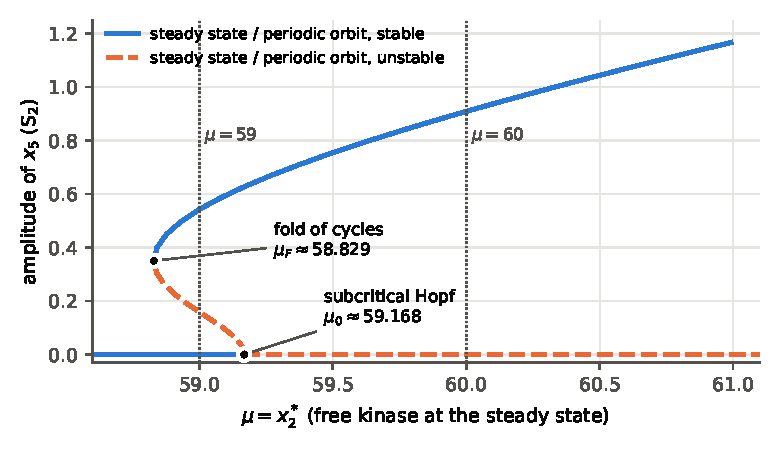
\includegraphics[width=0.82\textwidth]{figures/bifurcation.pdf}
\caption{Floating-point continuation of the periodic orbits along $\mu=x_2^*$ (rate constants $k^*$, $x_1^*=1/3$, $x_6^*=1/4$); amplitude of $x_5$ (doubly phosphorylated substrate). The unstable orbits born at the subcritical Hopf point $\mu_0$ turn at a fold of cycles $\mu_F\approx58.855$ into stable orbits that persist past $\mu_0$. For $\mu_F<\mu<\mu_0$ a stable steady state coexists with a stable and an unstable orbit. \zcref[S]{thm:explicit} certifies the two orbits at $\mu=59$; \zcref{prop:conj} certifies the stable orbit at $\mu=60$. The figure itself is an illustration, not part of any proof.}
\label{fig:bif}
\end{figure}

\section{Proof of \zcref{thm:hopf}}\label{sec:proofhopf}
\paragraph{The family.} For $\mu>0$ consider $\dot z=\mathcal F(z,\mu):=P\,g(x^*(\mu)+Ez)$. This is~\eqref{eq:reduced} for the class $T(\mu)$ written in the shifted coordinate $z-Px^*(\mu)$, a polynomial family in $(z,\mu)$ with $\mathcal F(0,\mu)=0$, $D_z\mathcal F(0,\mu)=A(\mu)$ and $D_z^2\mathcal F(0,\mu)=B$. A periodic orbit of $\dot z=\mathcal F(z,\mu)$ near $0$ is mapped by $z\mapsto x^*(\mu)+Ez$ to a periodic orbit of $\dot x=g(x)$ in the affine space $\{Wx=T(\mu)\}$ near $x^*(\mu)>0$, hence in $\mathcal P_{T(\mu)}\cap\mathbb R^9_{>0}$.

\paragraph{Step 1: the bifurcation point (exact arithmetic).} The certificate script of \zcref{sec:verif} computes $A(\mu)$, the coefficients $b_i\in\mathbb Q[\mu]$ and $H_1,\dots,H_5\in\mathbb Q[\mu]$ exactly, checks the identity $\det(\lambda I_9-Dg(x^*(\mu)))=\lambda^3\det(\lambda I_6-A(\mu))$ symbolically, and checks $H_5(a)H_5(b)<0$ in exact rational arithmetic. By the intermediate value theorem $H_5(\mu_0)=0$ for some $\mu_0\in(a,b)$.

\paragraph{Step 2: the spectrum at $\mu_0$ (ball arithmetic).} Evaluating the exact polynomials on the ball $[a,b]$ with Arb~\autocite{Arb2017} at 600 bits gives $H_1,\dots,H_4>0$, $b_6>0$ and $H_5'\ne0$ on $[a,b]$. By the criterion of Liu~\autocite{Liu1994} (see also Yang~\autocite{Yang2002} and~\autocite[Prop.~2.3]{CMS2019}), $A(\mu_0)$ has exactly one pair of purely imaginary eigenvalues $\pm i\omega_0$, which is simple, and the other four eigenvalues have negative real parts; with $H_5'(\mu_0)\ne0$ the pair crosses the imaginary axis transversally. As an independent check, $\omega_0^2$ is a root of $b_1s^2-b_3s+b_5$ (imaginary part of the characteristic polynomial at $i\omega_0$). Of its two roots, the enclosure of one makes the real part $-s^3+b_2s^2-b_4s+b_6$ contain~$0$ and the enclosure of the other excludes~$0$, which identifies $\omega_0^2=s_0$. The cofactor $\lambda^4+c_1\lambda^3+c_2\lambda^2+c_3\lambda+c_4=p(\lambda)/(\lambda^2+s_0)$, with $c_1=b_1$, $c_2=b_2-s_0$, $c_3=b_3-s_0c_1$, $c_4=b_4-s_0c_2$, satisfies the four Routh--Hurwitz inequalities, and the remainders $b_5-s_0c_3$, $b_6-s_0c_4$ contain~$0$. In floating point the other four eigenvalues are approximately $-4.17$, $-60.5$, $-88.8$, $-181.7$.

\paragraph{Step 3: eigenvectors, Lyapunov coefficient and crossing speed (ball arithmetic).} Let $M=A(\mu_0)-i\omega_0I$, which has rank~5. The right eigenvector $q$ normalised by $q_5=1$ is the unique solution of the $5\times5$ system obtained by deleting one row of $Mq=0$ and moving the column of $q_5$ to the right-hand side. That subsystem is nonsingular (its ball Gaussian elimination succeeds), and the deleted equation is a consequence of the other five because $\operatorname{rank}M=5$. Ball arithmetic therefore encloses $q$; the same construction for $M^{\mathsf T}$ encloses a left null vector $w$, and $\bar p:=w/(w^{\mathsf T}q)$ satisfies $\bar p^{\mathsf T}A=i\omega_0\bar p^{\mathsf T}$ and $\bar p^{\mathsf T}q=1$. Kuznetsov's projection formula~\autocite{Kuznetsov1999}, \autocite[§3.5 and Ch.~5]{Kuznetsov2004}, with the cubic term absent, gives the first Lyapunov coefficient
\begin{equation}\label{eq:l1}
\ell_1=\frac{1}{2\omega_0}\operatorname{Re}\Bigl[\bar p^{\mathsf T}\Bigl(-2B\bigl(q,A^{-1}B(q,\bar q)\bigr)+B\bigl(\bar q,(2i\omega_0I-A)^{-1}B(q,q)\bigr)\Bigr)\Bigr],
\end{equation}
with $A=A(\mu_0)$, which is invertible because $b_6>0$. Its sign does not depend on the normalisation of $q$ (rescaling $q$ by $c$ multiplies $\ell_1$ by $|c|^2$) nor on the choice of linear coordinates. The enclosure is
\[
\ell_1\in[5.86860833657\times10^{-4}\pm10^{-17}]>0 .
\]
For the simple eigenvalue $\lambda(\mu)$ with $\lambda(\mu_0)=i\omega_0$, $\lambda'(\mu_0)=\bar p^{\mathsf T}A'(\mu_0)q$, and the enclosure gives $\operatorname{Re}\lambda'(\mu_0)\in[0.00569698769645\pm3\cdot10^{-15}]>0$. The linear solves in~\eqref{eq:l1} are ball Gaussian eliminations, which enclose the exact solution for every matrix and right-hand side in the input balls; all inputs are balls containing the exact values at $(\mu_0,\omega_0)$, so the output encloses the exact $\ell_1$ and $\lambda'(\mu_0)$.

\paragraph{Step 4: the Hopf theorem.} The family $\mathcal F$ is polynomial, $A(\mu_0)$ has the simple pair $\pm i\omega_0$ and no other eigenvalue on the imaginary axis, $\alpha'(\mu_0)>0$ where $\alpha=\operatorname{Re}\lambda$, and $\ell_1>0$. In the notation of Hassard, Kazarinoff and Wan~\autocite[Ch.~1]{HKW1981}, $\operatorname{Re}c_1(0)=\omega_0\ell_1>0$ (\autocite[§3.5]{Kuznetsov2004}), so $\mu_2=-\operatorname{Re}c_1(0)/\alpha'(\mu_0)<0$ and $\beta_2=2\operatorname{Re}c_1(0)>0$. The Hopf bifurcation theorem in $\mathbb R^n$~\autocite[Ch.~1]{HKW1981}, see also~\autocite[§§3.4--3.5, with the centre manifold reduction of Ch.~5]{Kuznetsov2004}, gives $\delta>0$ and, for every $\mu\in(\mu_0-\delta,\mu_0)$, a unique nonconstant periodic orbit $\Gamma_\mu$ in a fixed neighbourhood of the origin. It shrinks to the origin as $\mu\uparrow\mu_0$, and its nontrivial characteristic exponent on the centre manifold is positive, so $\Gamma_\mu$ is unstable; the four other directions are contracting. For $\mu<\mu_0$ close to $\mu_0$ the eigenvalue pair has negative real part (Step~3) and the other four eigenvalues remain in the open left half-plane by continuity, so $x^*(\mu)$ is LAS. Mapping back by $z\mapsto x^*(\mu)+Ez$ proves \zcref{thm:hopf}. \qed

\section{Proof of \zcref{thm:explicit}}\label{sec:proofexplicit}
\paragraph{Local stability (exact).} At $\mu=59$, \eqref{eq:xstar} gives the stated rational $x^*>0$; $g(x^*)=0$ and $Wx^*=T(59)$ hold exactly. The exact Hurwitz determinants of $A(59)$ are all positive ($H_5=4.398\ldots\times10^{23}$) and $b_6>0$, so $x^*$ is LAS by the Routh--Hurwitz criterion. Arb's certified eigenvalue enclosures of the exact rational matrix agree: six eigenvalues with negative real part, the closest to the axis being $-0.000956948\ldots\pm2.24044\ldots i$.

\paragraph{The periodic orbits (CAPD).} We use the reduced system~\eqref{eq:reduced} for $T=T(59)$, the Poincaré section $\Sigma=\{z_5=c\}$ ($x_8=c$, with $c$ the double nearest to $5959/150$), crossed with $x_8$ increasing, and coordinates $y=(z_1,z_2,z_3,z_4,z_6)$ on $\Sigma$. The program \texttt{po\_proof.cpp} uses the CAPD library~\autocite{CAPD2021} (rigorous Taylor integration with the $C^1$ Lohner algorithm~\autocite{Zgliczynski2002}) to enclose the Poincaré map $\Pi$ at a numerically computed point $y_c$ and its derivative $D\Pi$ on a box $X\ni y_c$ of radius $10^{-8}(1+|y_{c,i}|)$. With $C\approx(D\Pi(y_c)-I)^{-1}$ it checks
\[
K(X)=y_c-C(\Pi(y_c)-y_c)+\bigl(I-C(D\Pi(X)-I)\bigr)(X-y_c)\subset\operatorname{int}X .
\]
By the Krawczyk theorem~\autocite{Krawczyk1969}, \autocite[§5.1]{Neumaier1990}, $\Pi$ then has a unique fixed point in $X$, that is, a periodic orbit of~\eqref{eq:reduced} crossing $\Sigma$ in $X$. The rate constants and totals enter as intervals that contain the exact rationals, and the program also checks that all nine concentrations are positive on $X$. The checks pass for two boxes:
\begin{itemize}
\item $X_s\ni(8.4587632,\,10.7368258,\,0.6108895,\,3.5188776,\,0.0302965)$: return time in $[2.969822982,\,2.969823054]$, $\|I-C(D\Pi(X_s)-I)\|_\infty\le0.067$;
\item $X_u\ni(9.3018468,\,10.2417384,\,0.2773832,\,3.3981275,\,0.0643781)$: return time in $[2.829105313,\,2.829105405]$, $\|I-C(D\Pi(X_u)-I)\|_\infty\le0.55$.
\end{itemize}
The two boxes are disjoint and each fixed point is a fixed point of the \emph{first} return map, so each orbit crosses $\Sigma$ upward only once per period; the two orbits are therefore distinct. Each orbit is positive at one point, hence everywhere, because $\mathbb R^9_{>0}$ is forward invariant and the orbit is periodic. Mapped by $\xi_T$, they are periodic orbits of $\dot x=g(x)$ in $\mathcal P_T$, and each return time is the minimal period, since the first return to $\Sigma$ is the point itself.

\paragraph{Stability of $\Gamma_s$.} With $S=\operatorname{diag}(1+|y_{c,i}|)$, the program computes the interval matrix $(S^{-1}D\Pi(X_s)S)^{128}$ by repeated squaring and finds $\infty$-norm at most $0.296$. Interval matrix multiplication is inclusion monotone, so for every matrix $D$ in the enclosure $\rho(D)\le\|(S^{-1}DS)^{128}\|_\infty^{1/128}<1$. In particular the derivative of $\Pi$ at its fixed point, whose eigenvalues are the five nontrivial Floquet multipliers of $\Gamma_s$, has spectral radius below~1. Hence $\Pi$ is a contraction near its fixed point $y_s$ in a suitable norm, and $\Pi^n(y)\to y_s$ for every $y$ in a neighbourhood $V\subset\Sigma$ of $y_s$. Every trajectory of~\eqref{eq:reduced} that starts close enough to $\Gamma_s$ crosses $\Sigma$ in $V$ within a bounded time, by continuity of the flow and transversality of $\Gamma_s$ to $\Sigma$. Continuity of the flow on bounded time intervals then shows that its distance to $\Gamma_s$ tends to~0. So $\Gamma_s$ is orbitally asymptotically stable within $\mathcal P_T$; by the Andronov--Witt theorem it even has an asymptotic phase (see e.g.~\autocite{Hartman1964}). Its basin is relatively open in $\mathcal P_T$, nonempty, and disjoint from the basin of $x^*$. \qed

In floating point, the nontrivial multipliers are about $0.9786$ for $\Gamma_s$ and $1.0044$ for $\Gamma_u$, the next ones being of order $10^{-5}$. So $\Gamma_u$ is a saddle orbit, presumably the continuation of the Hopf orbits of \zcref{thm:hopf} (\zcref{fig:bif}); neither fact is used in the proof.

\section{Proof of \zcref{thm:open}}\label{sec:proofopen}
Let $\mathcal B$ be the closed box $k\in k^*(1\pm\varepsilon)$, $y=(x_1,x_2,x_6)\in(\tfrac13,59,\tfrac14)(1\pm\varepsilon)$, $\varepsilon=10^{-12}$. The script \texttt{certify\_open\_set.py} checks:
\begin{enumerate}
\item $\det D_y(W\varphi_k)(y)\in[1806.708\pm10^{-4}]$ on $\mathcal B$, so $(k,y)\mapsto(k,W\varphi_k(y))$ is a local diffeomorphism there, and the image $U$ of the interior of $\mathcal B$ is open and nonempty;
\item with an approximate eigenvector matrix $R$ of $A$ at the centre (exact double entries), the Gershgorin discs of the ball matrix $R^{-1}A(k,y)R$ (enclosing $R^{-1}A(k,y)R$ for every $(k,y)\in\mathcal B$) lie in $\operatorname{Re}\lambda\le-9.56\times10^{-4}$, so every steady state $\varphi_k(y)$, $(k,y)\in\mathcal B$, is LAS;
\item the totals $W\varphi_k(y)$ over $\mathcal B$ lie in the boxes $K_{\rm tot}\in[78.666666667\pm5\cdot10^{-10}]$, $P_{\rm tot}\in[3.6261111111\pm4\cdot10^{-11}]$, $S_{\rm tot}\in[63.277592593\pm9\cdot10^{-10}]$;
\item \texttt{po\_proof\_box.cpp}, the variant of \texttt{po\_proof.cpp} in which the 13 parameters are additional constant state variables (so that the Lohner algorithm tracks their influence to first order), proves the Krawczyk inclusion and the spectral bound for $\Gamma_s$ simultaneously for all rate constants in $k^*(1\pm\varepsilon)$ and all totals in the boxes of item~3 ($\|I-C(D\Pi-I)\|_\infty\le0.36$).
\end{enumerate}
For $(k,T)\in U$, the steady state of $\mathcal P_T$ is $\varphi_k(y)$ for the corresponding $y$ (uniqueness, \autocite[Prop.~3.1]{CMS2019}), which is LAS by item~2, and $\mathcal P_T$ contains an orbitally asymptotically stable periodic orbit by item~4 and the argument of \zcref{sec:proofexplicit}. \qed

The width $\varepsilon=10^{-12}$ reflects only the cost of the interval method (the fixed point moves by roughly $10^{5}\varepsilon$ while the Krawczyk box must stay small); the floating-point continuation of \zcref{fig:bif} indicates a bistable window of relative width about $0.5\%$ in $\mu$ alone.

\section{How common is subcriticality?}\label{sec:numerics}
The following observations are floating point and are not used in any proof. All Hopf points were located as sign changes of the largest real part of the spectrum along $x_2$, and $\ell_1$ was evaluated with~\eqref{eq:l1}. That routine was validated against the planar Guckenheimer--Holmes formula and, for this model, by direct simulation at the Hopf point.
\begin{itemize}
\item For the rate constants of~\autocite[Table~1]{CMS2019}, all $494$ Hopf points found on a $50\times50$ grid of $(x_1,x_6)\in[10^{-4},10^4]\times[10^{-5},10^{4}]$ are supercritical, consistent with the Matcont observations of~\autocite[Figs.~2 and 4]{CMS2019}. The two Hopf points of their Figure~1 have $\ell_1<0$.
\item With log-uniform random rate constants restricted to the region of~\autocite[Thm.~4.2]{CMS2019} ($k_{10}$ above the bound~(13), $k_5/k_8$ large), $15\,929$ of $70\,884$ Hopf points ($22\%$) are subcritical; with unrestricted log-uniform rate constants on $[10^{-2},10^{2}]$, $44$ of $1\,259$.
\item For $k^*$ itself, about $8\%$ of the Hopf points found on a grid of $(x_1,x_6)$ are subcritical, so $\ell_1$ changes sign on the Hopf surface: there are generalised Hopf (Bautin) points.
\end{itemize}
Subcritical Hopf points are therefore not exceptional, but they are absent near the parameter values used in~\autocite{CMS2019}, which explains the simulations reported there.

\section{Conjecture 6.1}\label{sec:conj}
\zcref[S]{thm:hopf,thm:explicit} do not contradict Conjecture~6.1: they concern classes with a stable steady state. They do show that the stable/unstable dichotomy of the steady state is not a dichotomy between convergence and oscillation, because oscillations also occur in classes with a stable steady state. In our example, the unstable orbits born at the Hopf point fold into stable orbits that persist on the unstable side (\zcref{fig:bif}), as Conjecture~6.1 predicts. We certify one instance.

\begin{proposition}\label{prop:conj}
For $k=k^*$ and $T=T(60)=(80,\ 221/60,\ 5791/90)$ the steady state $x^*=(\tfrac13,60,10,10,\tfrac8{45},\tfrac14,\tfrac{10}3,\tfrac{202}5,\tfrac1{10})$ is unstable (exactly two eigenvalues with positive real part, $0.0047032\ldots\pm2.24702\ldots i$), and $\mathcal P_T$ contains an orbitally asymptotically stable periodic orbit (return time in $[3.09916969,\,3.09916978]$).
\end{proposition}
\begin{proof}
Exact Hurwitz determinants ($H_1,\dots,H_4>0$, $H_5<0$, $b_6>0$), certified Arb eigenvalue enclosures, and the CAPD proof of \zcref{sec:proofexplicit} with $\mu=60$ (\texttt{certify\_orbits.py}).
\end{proof}

Two remarks on what a proof of Conjecture~6.1 would need. First, when $k_2=k_6=k_9$, \autocite[Prop.~4.1]{CMS2019} gives $H_1,\dots,H_4>0$ and $b_6>0$ at every steady state. By Routh's theorem~\autocite[Ch.~XV]{Gantmacher1959}, a steady state that is not LAS and not on the Hopf surface ($H_5<0$) then has exactly two eigenvalues in the open right half-plane and none on the axis, hence a two-dimensional unstable manifold in its class; in $3\times10^5$ random floating-point samples, with unequal dissociation constants allowed, we never observed more than two. Second, the conjecture is a global statement about all classes with an unstable steady state, including those far from any Hopf point. Our methods certify individual orbits but give no handle on, for instance, excluding a stable invariant torus or a chaotic attractor without stable periodic orbits. We did not search systematically for such attractors. Conjecture~6.1 remains open.

\section{Computer verification}\label{sec:verif}
All scripts are in \texttt{scripts/} and print PASS or FAIL for every claim, with a non-zero exit code on failure (Python~3.12, SymPy~1.14, python-flint~0.9; CAPD~6.1 built from \url{https://github.com/CAPDGroup/CAPD} in WSL Fedora).
\begin{itemize}
\item \texttt{certify\_subcritical\_hopf.py} (8~s): claims C0--C8 of \zcref{thm:hopf}: conservation laws; the parametrisation (symbolic in all $k_i$ and $x_1,x_2,x_6$); the reduction identity $\lambda^3p_A$; the exact sign change of $H_5$; ball checks of $H_1,\dots,H_4$, $b_6$, $H_5'$; identification of $\omega_0$ and the Hurwitz cofactor; $\ell_1>0$; $\operatorname{Re}\lambda'>0$; the totals~\eqref{eq:Tmu}. Data: \texttt{certificates/hopf\_point.json}, generated by \texttt{make\_hopf\_point.py}.
\item \texttt{certify\_orbits.py} (about 40~s, mostly compilation): exact steady states, Hurwitz determinants and Arb eigenvalue enclosures at $\mu=59,60$; a symbolic check that the vector field typed in \texttt{po\_proof.cpp} equals $P\,g(\xi_T(z))$ for symbolic $k$ and $T$; compilation and runs of \texttt{po\_proof} for the three orbits, with rationals enclosed by outward-rounded doubles. Data: \texttt{certificates/orbits.json}; log: \texttt{certificates/po\_proof\_log.txt}.
\item \texttt{certify\_open\_set.py} (about 1~min): items 1--4 of \zcref{sec:proofopen}; its log is \texttt{certificates/\allowbreak open\_set\_log.txt}.
\item \texttt{exploration/}: the floating-point searches, continuation and figure (not certificates).
\end{itemize}

\paragraph{Assumptions and limitations.} The proofs rely on: the uniqueness of the steady state in each class~\autocite[Prop.~3.1]{CMS2019} (only for the word ``unique'' and in \zcref{thm:open}); the Hopf theorem with the stability formula of~\autocite{HKW1981} and the projection formula~\eqref{eq:l1}~\autocite{Kuznetsov1999,Kuznetsov2004}; Liu's criterion~\autocite{Liu1994}; the Krawczyk theorem; and the correctness of the Arb, FLINT and CAPD implementations of interval arithmetic and rigorous integration. \zcref[S]{thm:hopf} gives no explicit~$\delta$; \zcref{thm:explicit} is the quantitative counterpart. The value $\mu_F$ of the fold of cycles, the amplitudes in \zcref{fig:bif}, the statements of \zcref{sec:numerics} and the identification of $\Gamma_u$ with the Hopf orbits are numerical and not proved.

\paragraph{Related work.} We found no computation of Lyapunov coefficients for this network. Vassena~\autocite{Vassena2026} and Feliu and Kaihnsa~\autocite{FK2024} concern the fully distributive network. The Evidence Press record~\autocite{Zenodo23446981} treats reduction conjectures of~\autocite{FK2024} and states that it does not resolve the dual-phosphorylation question.

\paperreferences
\end{document}
